% slide maggiormente teoriche e metodologiche sul modello testo e modello di markup

% slide del turco, slide vitali, argomenti deRose, paper su Bellisage
% http://xml.coverpages.org/DeRoseEML2004.pdf
% libro ciotti aracne Testo e automi: https://core.ac.uk/download/pdf/53833252.pdf
% Domenico Fiormonte (slide)

%introdurre alcuni problemi teorici generali, che costituiscono la base delle nostre ricerche.


% Non poteva dunque rimanere immune da tale pervasiva influenza il sapere umanistico e letterario.

% Modello della comunicazione dell'informazione (vedere libro google play)
% modello OHCO e altro (What text really is, inadequacy of markup)
% linguaggi di Markup
% prospettiva documento centrica e prospettiva data centrica


\documentclass{beamer}
    
%    \usepackage[english]{babel}
    %\usepackage[latin1]{inputenc}
    %\usepackage[T1]{fontenc}

\mode<presentation>{
  \setbeamertemplate{background canvas}[vertical shading]
  \usetheme{Berkeley}
  \useoutertheme{himinfolines}
}
  
\usepackage{ucs}
\usepackage[utf8]{inputenc}
\usepackage[english,polutonikogreek,italian,UKenglish,british]{babel}
\usepackage{graphicx}
\usepackage{colortbl}
\usepackage{multicol}
\usepackage{ulem}
\usepackage{verbatim}
\usepackage{alltt}
\usepackage{ccicons}
\usepackage{MnSymbol,wasysym}
\usepackage{tikzsymbols}
\usepackage{textcomp}
\usepackage{xmpincl}

\usepackage{parskip}
\setcounter{nframes}{100}
\setcounter{nframe}{1}
\setbeamercovered{dynamic}
\newenvironment{grcenv}{\begin{otherlanguage}{greek}}{\end{otherlanguage}}
\newcommand{\g}[1]{\textgreek{#1}}
\definecolor{darkgreen}{rgb}{0,0.5,0}
\definecolor{darkblue}{rgb}{0,0,0.5}
\definecolor{grey}{rgb}{0.5,0.5,0.5}
\setcounter{tocdepth}{5}

\makeatletter

\makeatother
%\includexmp{LicencesAndLicensing}

%frame00 metadata
    \title{Codifica di Testi - Introduzione Teorica \\a.a. 2018-2019}
    \author[A.M. Del Grosso]{Angelo Mario Del Grosso}
    \institute{\texttt{angelo.delgrosso@ilc.cnr.it} \\\bigskip\textit{CNR-ILC-LicoLab}}
    \date{Istituto di Linguistica Computazionale ``A. Zampolli'', \today}
    \AtBeginSection[]{
    \begin{frame}<beamer>
    \addtocounter{nframe}{1}
    \footnotesize
    \frametitle{Progress status}
    \tableofcontents[currentsection,hideothersubsections]
    \end{frame}
    }

\begin{document}

\begin{frame}
	\maketitle
\end{frame}

\begin{frame}
	\frametitle{Contenuto della lezione}
	\tableofcontents
\end{frame}

\section{Elementi Teorici e Metodologici della codifica}
\begin{frame}
	\frametitle{Codifica e Modellizzazione}
	\framesubtitle{Problemi e opportunità}
	\addtocounter{nframe}{1}

	\begin{block}{Il testo, oggetto di studio}
		%
\includegraphics[width=.5\textwidth]{../imgs/tei-r.pdf}
		Le discipline umanistiche hanno come oggetto di studio privilegiato i testi.
		\\ L'avvento delle tecnologie informatiche ha cambiato la produzione, la trasmissione e lo studio del sapere e della conoscenza (quindi anche il testo).
	\end{block}

	\begin{block}{Il testo in ambiente digitale}
		Il nuovo formato digitale ha determinato profonde trasformazioni nelle pratiche scientifiche che hanno per oggetto o fine i testi.
	\end{block}


\end{frame}

\begin{frame}
	\frametitle{Codifica e Modellizzazione}
	\framesubtitle{Problemi e opportunità}
	\addtocounter{nframe}{1}

	\begin{block}{Vero e proprio cambio di paradigma}
		Gli studiosi si sono interrogati sul nuovo rapporto che le discipline umanistiche devono avere con il testo che diventa elettronico o digitale.
	\end{block}

	\begin{block}{Nuove sfide}
		La natura del formato digitale ha aperto nuove sfide  al fine di determinare e trovare soluzioni ai problemi connessi alla rappresentazione formale dei testi.
	\end{block}


\end{frame}


\begin{frame}
	\frametitle{Codifica e Modellizzazione}
	\framesubtitle{Problemi e opportunità}
	\addtocounter{nframe}{1}

	\begin{block}{Discussione nella comunità}
		L'informatica allo stato attuale è in grado di fornire allo studioso di scienze umane una serie di tecnologie per implementare dei sistemi di rappresentazione testuale.
	\end{block}

	\begin{block}{Nuove sfide}
		La discussione sulla rappresentazione digitale dei testi ha rivelato un intreccio di complesse questioni teoriche e pratiche
	\end{block}

\end{frame}

\begin{frame}
	\frametitle{Definizione di codifica informatica dei testi}
	\framesubtitle{Fabio Ciotti 2007}
	\addtocounter{nframe}{1}

	\begin{block}{Definizione}
		Per \textbf{codifica} informatica dei testi intendiamo la \textit{rappresentazione formale} di un \textbf{testo} ad un qualche livello descrittivo, su di un supporto digitale, in un formato utilizzabile da un elaboratore (\textit{Machine Readable Form}) mediante un opportuno \textbf{linguaggio informatico}
	\end{block}

\end{frame}


\begin{frame}
	\frametitle{Concetti alla base della codifica di testi}
	\framesubtitle{Gli elementi}
	\addtocounter{nframe}{1}

    \begin{itemize}
        \item Cosa significa Codifica
        \item Cosa significa Testo
        \item Cosa significa Codifica del Testo
        \item Cosa significa Linguaggio Informatico
    \end{itemize}

\end{frame}

\section{Codifica del Testo}
%% vedere slide Chiara di Pietro e Rosselli del turco.
\begin{frame}
	\frametitle{La comunicazione Umana}
	\framesubtitle{per comprendere la codifica bisogna partire da lontano}
	\addtocounter{nframe}{1}

	\begin{block}{In principio c'è la comunicazione}
		Comunicare è la facoltà di trasmettere qualcosa a qualcuno. Per comunicare bisogna condividere un sistema di referimento.
		\\(Comunicare deriva dal latino communis che indica proprio la condivisione)
	\end{block}

	\begin{block}{Primo schema di base di un sistema di comunicazione}
		Qualcuno/Qualcosa che Produce; Qualcuno/Qualcosa che Trasmette; Qualcuno/Qualcosa che Consuma
	\end{block}

\end{frame}

\begin{frame}
	\frametitle{La comunicazione Umana}
	\framesubtitle{Modello della Comunicazione - C. Shannon e W. Weaver (1949)}
	\addtocounter{nframe}{1}

	\begin{center}
		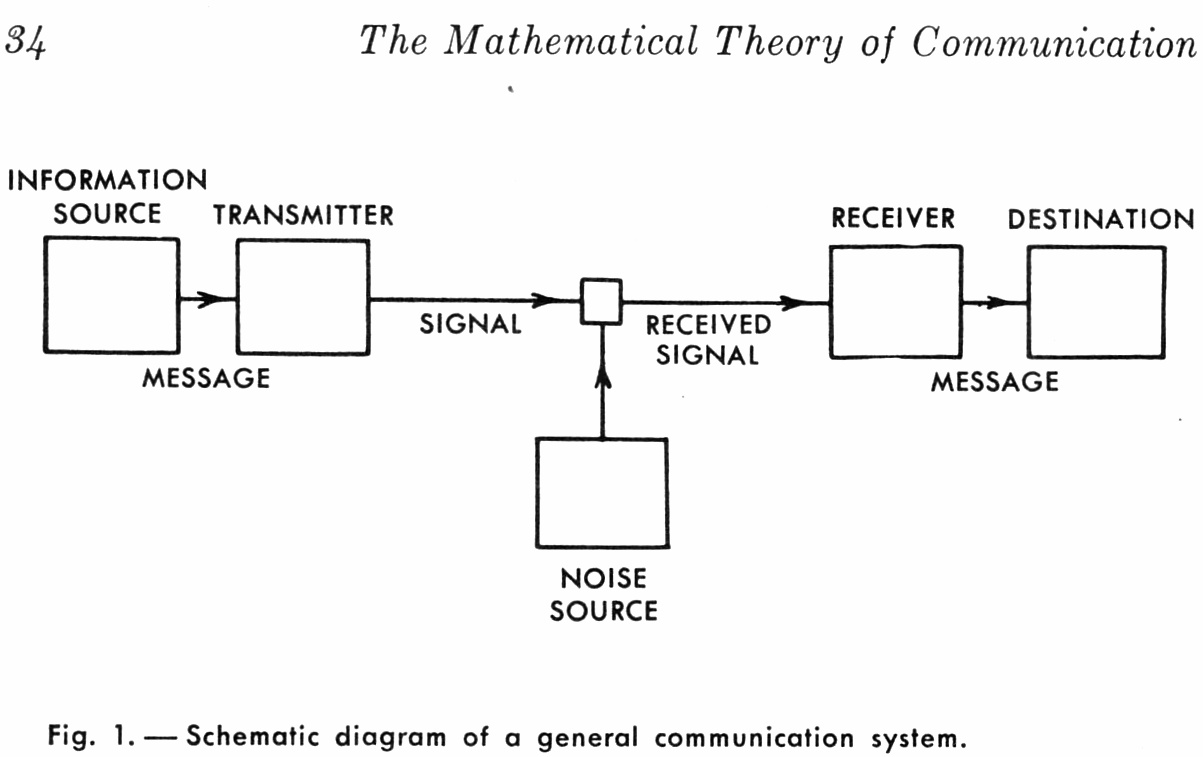
\includegraphics[width=.9\textwidth]{imgs/shannon_comm_channel.jpg}
	\end{center}

\end{frame}

\begin{frame}
	\frametitle{La comunicazione Umana}
	\framesubtitle{Modello della Comunicazione -Roman Jakobson (1966)}
	\addtocounter{nframe}{1}

	\begin{center}
		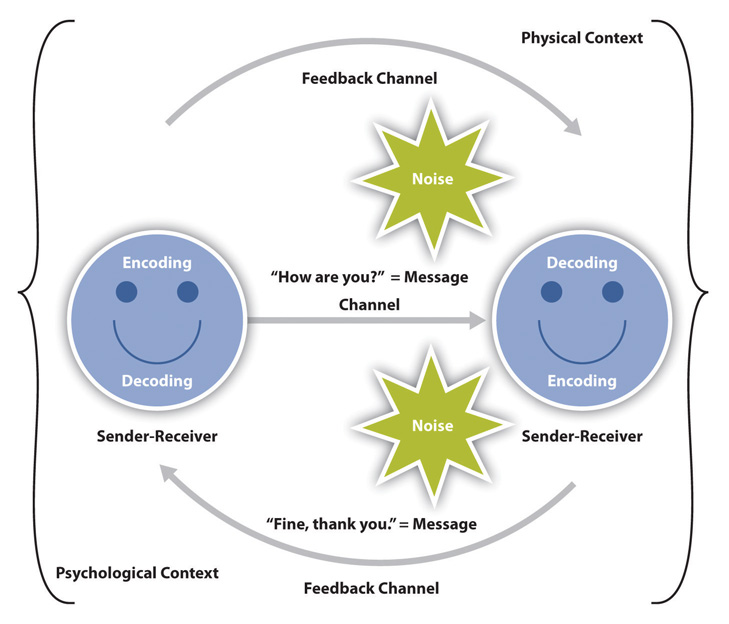
\includegraphics[width=.73\textwidth]{imgs/RomanJakobson.jpg}
	\end{center}
	\noindent\rule{5cm}{0.01cm}
	\\\tiny\url{http://open.lib.umn.edu/}

\end{frame}

\begin{frame}
	\frametitle{La comunicazione Umana}
	\framesubtitle{R. Jakobson}
	\addtocounter{nframe}{1}

	\begin{block}{Estratto Linguistics and Poetics}
		\textit{“The addresser sends a message to the addressee. To be
			operative the message requires a context referred to
			('referent' in another, somewhat ambivalent, nomenclature),
			seizable by the addressee, and either verbal or capable of
			being verbalized, a code fully, or at least partially, common to
			the addresser and addressee (or in other words, to the
			encoder and decoder of the message); and finally, a contact,
			a physical channel and psychological connection between the
			addresser and the addressee, enabling both of them to stay in
			communication.” (R. Jakobson, ‘Closing Statement:
			Linguistics and Poetics’, in Sebeok, Thomas A (Ed.) (1960):
			Style in Language. Cambridge, MA: MIT Press, p. 353)}
	\end{block}

\end{frame}

\begin{frame}
	\frametitle{La comunicazione Umana}
	\framesubtitle{R. Jackobson}
	\addtocounter{nframe}{1}

	\begin{block}{Modello Comunicazione: Funzione e Fattore}
		\textbf{Funzione}        \textbf{Fattore}
		\\Referenziale    Contesto
		\\Espressiva      Mittente
		\\Conativa        Destinatario
		\\Fàtica          Contatto
		\\Metalinguistica Codice
		\\Poetica         Messaggio
	\end{block}

\end{frame}

\begin{frame}
	\frametitle{La comunicazione Umana}
	\framesubtitle{Diasistema}
	\addtocounter{nframe}{1}

	\begin{block}{Messaggio}
		Nel sistema della comunicazione umana non c'è una assoluta corrispondenza tra il sistema di codifica e il sistema di decodifica.
		\begin{center}
			\textit{Codice dell'agente emittente è diverso dal codice dell'agente destinatario}
		\end{center}
	\end{block}

	\begin{block}{Messaggio}
		\begin{center}
			M\textsubscript{e} != M\textsubscript{d}
			\textbf{Il Messaggio codificato è diverso dal messaggio decodificato}
		\end{center}
	\end{block}

\end{frame}

\begin{frame}
	\frametitle{La comunicazione Umana}
	\framesubtitle{Diasistema}
	\addtocounter{nframe}{1}

	\begin{block}{Diasistema - Weinreich, Uriel. - Linguista (Vilna, Polonia, 1926 - New York 1967)}
		Sistema (linguistico) di livello superiore, che riunisce due o più sistemi omogenei tra i quali ci siano somiglianze parziali (sul piano fonematico, morfologico, lessicale).
	\end{block}

	\begin{block}{Messaggio}
		Il sistema di codifica e il sistema di decodifica sono due sottosistemi di uno stesso diasistema.
	\end{block}

\end{frame}

\begin{frame}
	\frametitle{La comunicazione Umana}
	\framesubtitle{Diasistema}
	\addtocounter{nframe}{1}

	\begin{block}{Comunicazione come diasistema}
		\begin{center}Comunicazione = Sistema dell'emittente (S1) $\sim$  Sistema del destinatario (S2).\end{center}
		\textit{Il risultato di compromesso tra il sistema S1 e il sistema S2}*
	\end{block}

	\rule{7cm}{0.015cm}
	\\*\tiny\textit{Segre, 1985}
\end{frame}

\begin{frame}
	\frametitle{Codifica del testo}
	\framesubtitle{Elementi del modello della comunicazione}
	\addtocounter{nframe}{1}

	\begin{block}{Codifica e Decodifica}
		\begin{itemize}
			\item Il termine codifica (in inglese \textit{encoding}) può essere associato alla creazione di un testo
			\item Il termine decodifica (in inglese \textit{decoding}) può essere associato alla comprensione e interpretazione di un testo
			\item Il messaggio può essere visto come contenitore di significato ($\sim$ \textit{testo})
		\end{itemize}
	\end{block}

\end{frame}

\begin{frame}
	\frametitle{Codifica del testo}
	\framesubtitle{definizioni}
	\addtocounter{nframe}{1}

	\begin{block}{Codice}
		Sistema di regole e di segni per convertire informazioni da una forma (anche astratta) in un'altra forma o rappresentazione per la comunicazione tramite un canale.
	\end{block}

\end{frame}

\begin{frame}
	\frametitle{Codifica del testo}
	\framesubtitle{Quando il destinatario è un calcolatore elettronico?}
	\addtocounter{nframe}{1}

	\begin{block}{La codifica informatica}
		Il codice deve essere in comune tra l'autore e la macchina, in un formato comprensibile ad entrambi.
	\end{block}

	\begin{block}{La codifica informatica}
		\begin{itemize}
			\item Codice in formato \textit{machine readable} (MRF), cioè un codice in formato comprensibile ad un calcolatore elettronico.
			\item Codificare per il computer implica una ricodifica del testo affinchè vengano esplicitate le caratteristiche e le funzioni del testo identificate.
		\end{itemize}
	\end{block}

\end{frame}

\begin{frame}
	\frametitle{Codifica del testo}
	\framesubtitle{Esplicitare in modo formale}
	\addtocounter{nframe}{1}

	\begin{block}{La codifica informatica}
		Codificare in formato digitale un testo significa esplicitare i processi inferenziali effettuati da un interprete nella comprensione del testo stesso.
	\end{block}


\end{frame}


\begin{frame}
	\frametitle{Codifica del testo}
	\framesubtitle{Sinteticamente}
	\addtocounter{nframe}{1}

	\begin{block}{La codifica digitale di un testo}
		la codifica testuale è la rappresentazione formale di un testo e delle sue caratteristiche mediante un linguaggio informatico. (Ciotti)
	\end{block}

	\begin{block}{Grammatica formale}
		Questo linguaggio consente di rappresentare esplicitamente le caratteristiche di un testo applicando etichette meta-testuali la cui funzione e applicazione è descritta da una grammatica formale (per essere ``comprese'' da una macchina/sistema software).
	\end{block}
\end{frame}

\begin{frame}
	\frametitle{Codifica del testo}
	\framesubtitle{Linguaggio formale che diventa linguaggio teorico}
	\addtocounter{nframe}{1}

	\begin{block}{La codifica del testo come modello formale}
		La codifica digitale del testo diviene a questo punto un linguaggio teorico attraverso il quale lo studioso costruisce modelli formali del testo.
	\end{block}

	\begin{block}{Linguaggi di Markup}
		Ai fini della modellizzazione di testi, tra i linguaggi formali si sono imposti quei sistemi basati sui cosiddetti linguaggi di marcatura (\textit{markup language}).
	\end{block}
\end{frame}


\begin{frame}
	\frametitle{Codifica del testo}
	\framesubtitle{Sistema linguistico formalizzato}
	\addtocounter{nframe}{1}

	\begin{block}{Secondo Lou Burnard 1995}
		La codifica informatica di un testo impone l'adozione di un sistema linguistico formalizzato che permetta a uno studioso di rendere esplicita una interpretazione di un testo e le varie operazioni che la hanno prodotta.
	\end{block}

	\begin{block}{I sistemi dichiarativi}
		\begin{center}
			\textbf{I sistemi dichiarativi forniscono un potente dispositivo metalinguistico.}
		\end{center}
	\end{block}

\end{frame}

%Fare la codifica di un testo significa
%convertirlo in un formato comprensibile per
%l’elaboratore
%usare, a tal fine, un linguaggio di codifica di tipo
%formale
%definire e seguire uno schema di codifica ben preciso
%stabilito in base alle caratteristiche del testo che si
%intende esplicitare per il computer (modello di codifica)



%Non è codifica di un testo
%fare una scansione di un documento e diffonderne le
%immagini (ad es. in formato PDF) → digitalizzazione
%usare un software OCR per ricavarne una versione in
%formato ASCII (anche se si tratta di MRF)
%creare una pagina HTML sulla base di tale testo ASCII
%creare un documento Word ...
%creare un database testuale sulla base di tale testo
%ASCII

\begin{frame}
	\frametitle{Codifica del testo}
	\framesubtitle{Finalità}
	\addtocounter{nframe}{1}

	\begin{block}{Prerequisito per una corretta rappressentazione digitale dei testi}
		Definizione e implementazione di un linguaggio formale che deve essere sia processabile da un computer sia sufficientemente espressivo per rappresentare la complessità del testo.
	\end{block}

	\begin{block}{Capacità rappresentazionale}
		\begin{center}
			\textbf{Il principale requisito di uno schema di codifica, pertanto, è la capacità rappresentazionale che esso offre allo studioso}
		\end{center}
	\end{block}

\end{frame}



\section{Modello del Testo}
% 	    %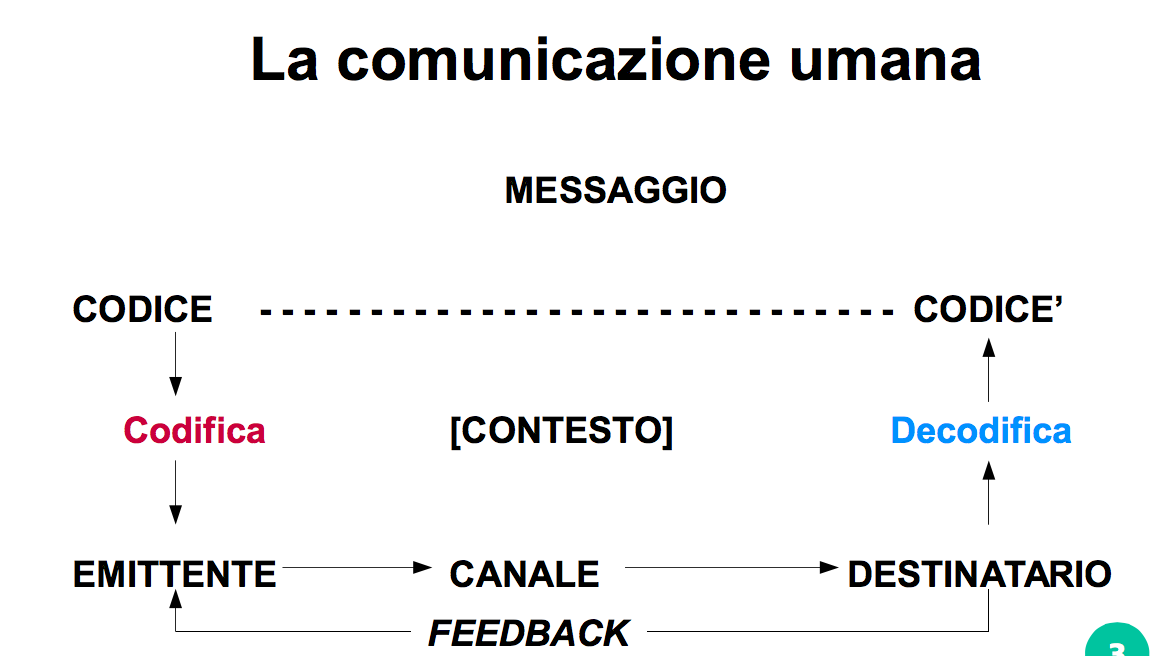
\includegraphics[width=.5\textwidth]{../imgs/comunicazioneUmana.png}




% L’applicazione di tecnologie informatiche nelle discipline umani- stiche, e in particolare nelle scienze letterarie, ha come suo fondamento la rappresentazione degli oggetti che costituiscono il loro dominio di studio. Tali oggetti sono in linea generale i testi.

% l’analisi del processo di scoperta e rappresentazione dell’oggetto testo e della sua struttura non può prescindere da una de- terminazione di cosa si intenda per testo, o quantomeno da una assun- zione implicita sulla sua natura;

% Il testo è un oggetto complesso in quanto è in grado di veicolare si- gnificato (e di rivestire dunque interesse scientifico) su più livelli strutturali, anche attraverso l’instaurazione di molteplici relazioni tra più livelli.

% Non possediamo nessuna teoria sufficientemente completa del testo

% Il fatto è che la rappresentazione (e a maggior ragione l’elaborazione) informatica è ontologicamente formale in senso stret- to.

% Il termine “testo”  si riferisce a un oggetto complesso e plurale, in cui esiste 
%- un livello materiale, il supporto e le tracce d’inchiostro, 
%- un livello astratto, la sequenza verbale, la quale a sua volta genera una serie di livelli di contenuti semantici.

% Lo studio del sapere ha come oggetto immediato i testi (letterari e non). Nella nostra cultura la quasi totalità dei testi letterari (fino a questo momento) è costituita da testi scritti su supporti cartacei di varia natura e forma.

% A questa struttura rigida del codice nell’ambito informatico (codice binario) va confrontata la complessa intersezione di codici che costituiscono un testo (da memorizzare).

% il termine “testo” non denota una entità acritica, oggetto della memorizzazione, affermando banalmente si tratta di una entità informativa complessa.

% Molteplici teorie del testo, quasi tutte sbilanciate sul livello verbale-semantico (linguistica testuale)

% Possiamo concludere che il testo è l’invariante, la successione di valori, rispetto alle variabili dei caratteri, della scrittura.
% Il testo è dunque una successione fissa di significati grafici (Segre, 1985).

% il testo come una entità astratta invariante, che in ogni operazione di realizzazione materiale della sequenza di simboli grafici determina la struttura fisica di un og- getto sensibilmente concreto (ovvero capace di attivare uno dei canali recettivi dell’uomo verso stimoli esterni), che costituisce il supporto materiale, stabile e riproducibile dell’informazione testuale. Distin- gueremo questo oggetto dal testo chiamandolo documento.

% Testo vs Documento

% oltre alla sequenza di grafemi, a un testo nel senso da noi indicato possono essere ascritte anche le segmentazioni logiche e le partizioni interne di interi blocchi
% il testo ha una certa struttura, i cui elementi sono determinati dalla struttura logico semantica del discorso,

% esiste anche un modello documento
% possibilità significative che derivano da una semantizzazione esplicita degli elementi non verbali di un testo scritto.
% ruolo della disposizione tipografica e topografica del segno grafico nella pagina bianca

% quale concezione o modello ontologico del testo è implicata nella rappresentazione informatica?

% natura del testo: il testo è, in un senso importante, una “ordered hierarchy of content objects (OHCO)”, una gerarchia ordinata di oggetti di contenuto [DeRose et al., 1990:3]. Gli oggetti di contenuto testuale a cui si fa riferimento in questa teoria sono sostanzialmente le strutture editoriali astratte di cui si com- pone un testo. Essi sono gerarchici poiché alcuni degli oggetti testuali con- tengono altri, e ordinati in quanto esiste una relazione lineare tra due oggetti posti sul medesimo livello gerarchico.

% il genere determina gli elementi che costituiscono il testo, quindi il tipo di documento. Reciprocamente un genere testuale è individuato dalla classe di oggetti di contenuto che contiene.
% Su questo impianto teorico si è basata, ad esempio, la prima fase del lavoro della Text Encoding Initiative.
% Sono però stati riscontrati una serie di problemi di rappresentazione che costituiscono dei veri e propri controesempi. Ci sono moltissimi casi in cui non esiste assolutamente accordo tra gli specialisti dei testi nell’asserire l’appartenenza di un dato testo a un tipo piuttosto che a un altro.  Questi diversi insiemi di elementi di contenuto non possono essere ricondotti a una struttura gerarchica unitaria.

% classi di elementi testuali che si sovrappongono rompendo i confini della struttura gerarchica di un documento: esempio: struttura metrica e quella morfosintattica di un testo poetico.. (Esempio clavius righe e sentence). Questi elementi si comportano come se appartenessero a diverse gerarchie di oggetti testuali che si sovrappongo.
% Prospettiva analitica:  “ogni prospettiva analitica su un testo determina una struttura gerarchica di oggetti di contenuto”.
% Un corollario operativo di questa tesi è che se due elementi a e b si sovrappongono, allora essi appartengono a due diverse prospettive analitiche.

% Ma è vero che a ogni coppia di elementi che si sovrappongono cor- rispondono due distinte prospettive teoriche? occorrenza di alcuni oggetti testuali che, pur appartenendo ragionevolmente a una medesima pro- spettiva analitica si sovrappongono.
%Se due oggetti testuali evidenziati da una prospettiva teorica si sovrap- pongono, allora essi appartengono rispettivamente a due sottoprospet- tive diverse della prospettiva teorica principale. Questa ultima revisione della teoria gerarchica abbandona qualsiasi assunto di tipo essenzialista. In questa ottica il testo diventa un sistema a più livelli, che corrispondono a diversi punti di vista dell’osservatore.
% • il testo è un oggetto reale dotato di una sua struttura che corrisponde alla struttura del linguaggio di rappresentazione;
% • la struttura o meglio le strutture del testo sono strutture gerar- chiche: le sottoprospettive, comunque esse siano definite, dan- no luogo a gerarchie.

% Alcune teorie avanzano la necessità di abbandonare l’assunto ontologico che il testo sia un oggetto reale del mondo, dotato di una struttura intrinseca: Il testo è dunque una entità che viene costruita e non scoperta e a- nalizzata dalla attività scientifica. soluzione interessante e intellettualmente stimolante alle aporie determinate dal- la teoria gerarchica del testo, specialmente nella tematizzazione del ruolo dell’osservatore nei processi di rappresentazione.

% cos'è il testo (uso comune):
%a) un documento materiale composto da fogli di carta rilegati (o spillati o semplicemente raccolti insieme da un nastro di carta) che contengono tracce di inchiostro variamente disposte (oltre a eventuali tracce di altri materiali)
%b) un discorso linguistico fissato tramite la scrittura su un docu- mento materiale
%c) un’opera dell’ingegno che viene costituita da quel discorso

% cos'è un testo (uso più specialistico)
% d) lo stato linguistico di un singolo testimone materiale di un’opera
% e) lo stato linguistico di un medesimo testimone di un’opera che presenta diverse lezioni identificabili
% f) una versione edita di un’opera
% g) una sequenza coerente di enunciati in una lingua naturale
% Teso è l'invariante rispetto ai segni, è la succesione di valori invariabili. Il testo, dunque è ciò che permane, l’invariante, in ogni operazione di riproduzione materiale della sequenza di simboli grafici.
% Questa definizione di testo come un oggetto astratto allografico sembra fornire un criterio di individuazione di un testo in base al prin- cipio di identità per sostituzione

%OHCO: alla do- manda che cosa è un testo veramente rispondiamo che un testo è un oggetto linguistico astratto organizzato secondo una struttura gerar- chica ordinata di oggetti di contenuto. (Asserzione poi rilevatasi fallace). Ma l’idea di una preminenza della struttura gerarchica nella testualità ha mantenuto un ruolo descrittivo ed esplicativo essenziale.

\section{Importanza della Codifica}
%% Vedere Slide CHiara. Roberto
% Portabilità e riutilizzabilità
% schema di codifica
% TEI XML focuses on the meaning of text, rather than its appearance.

\begin{frame}
	\frametitle{Importanza della codifica digitale}
	\framesubtitle{Perché effettuare la codifica}
	\addtocounter{nframe}{1}

	\begin{block}{Digitalizzare un testo}
		Digitalizzare per poter favorire l'elaborazione e il trattamento automatico dei testi
	\end{block}

	\begin{block}{Trattamento dei testi}
        \begin{itemize}
            \item  analisi di tipo linguistico (linguistica computazionale,
            database testuali, corpora linguistics)
            \item analisi di altro tipo (metrica, stilistica, etc.)
            \item ricerca testuale avanzata
            \item pubblicazione in vari formati (sul web, come ebook, a
            stampa)
            \item didattica
        \end{itemize}
 
    \end{block}
\end{frame}

\begin{frame}
	\frametitle{Importanza della codifica digitale}
	\framesubtitle{Perché effettuare la codifica}
	\addtocounter{nframe}{1}

	\begin{block}{Digitalizzare un testo}
		Per facilitare e garantire una universalità di accesso al loro contenuto 
	\end{block}

	\begin{block}{Vantaggi della digitalizzazione}
        \begin{itemize}
            \item Edizioni elettroniche garantiscono diffusione capillare
            (via web) e nuove funzionalità (ipertesti, ricerca, etc.)
            \item Permettono anche di preservare i documenti più antichi
            (e fragili) riducendone la consultazione diretta
        \end{itemize}
     \end{block}
\end{frame}

\begin{frame}
	\frametitle{Importanza della codifica digitale}
	\framesubtitle{Perché effettuare la codifica}
	\addtocounter{nframe}{1}

	\begin{block}{Superare i problemi dei documenti digitali}
		\begin{itemize}
            \item disponibilità di hardware e software
            \item sistemi proprietari chiusi
            \item elevata obsolescenza e limitata manutenibilità
            \item difficile portabilità su piattaforme diverse
        \end{itemize}
	\end{block}
	
\end{frame}

\begin{frame}
	\frametitle{Importanza della codifica digitale}
	\framesubtitle{Perché effettuare la codifica}
	\addtocounter{nframe}{1}

	\begin{block}{Sistemi non adatti}
		\begin{itemize}
            \item word processing: WYSIWYG (What You See Is What You Get)
            \item sistemi proprietari chiusi (Word, Adobe, etc)
            \item elevata obsolescenza e limitata manutenibilità
            \item difficile portabilità su piattaforme diverse (windows, linux)
        \end{itemize}
	\end{block}
	
\end{frame}

\begin{frame}
	\frametitle{Importanza della codifica digitale}
	\framesubtitle{Perché effettuare la codifica}
	\addtocounter{nframe}{1}

	\begin{block}{Massimizzare le seguenti proprietà: Portabilità}
		\begin{itemize}
            \item indipendenza dall’hardware: processore, supporto, output
            \item indipendenza dal software: sistemi operativi, applicazioni di authoring, applicazioni di visualizzazione
            \item indipendenza dai sistemi di codifica dei caratteri
            \item indipendenza logica: da un particolare processo applicativo
        \end{itemize}
	\end{block}
	
\end{frame}




%La codifica dell’informazione gode delle seguenti proprietà:
% indipendenza dall’hardware, ovvero da una particolare architettura elaborativa (processore), da un particolare supporto digitale (disco magnetico, disco ottico, etc.), o da un particolare dispositivo o sistema di output (video, stampa);
% indipendenza dal software, sia sistemi operativi, sia applicazioni deputate alla creazione, analisi, manipolazione e visualizzazione di testi elettronici; (formati di dati proprietari mutamente incompatibili)
% indipendenza logica dalle applicazioni ovvero indipendenza semantica dello schema di codifica da un particolare processo applicativo.

% L’archiviazione su supporto digitale del patrimonio letterario e culturale delle culture mondiali deve misurarsi con questi problemi, e adottare degli schemi di codifica capaci di garantire la massima portabilità. 



% Una risorsa informativa digitale è portabile se è intercambiabile tra sistemi diversi, riutilizzabile in molteplici processi computazionali anche a distanza di tempo, e integrabile da ulteriori risorse informative omogenee


%  Esso deve divenire uno standard
% I vantaggi di uno standard formale o informale, oltre alla portabilità sta anche nella sua apertura, ovvero nella disponibilità pubblica delle sue specifiche.



% La disposizione alla rappresentazione di strutture astratte non pone limiti alla natura e tipologia delle caratteristiche testuali che si possono codificare in un testo elettronico. Queste possono essere utilizzate indifferentemente 

% Se il linguaggio è dotato di una sintassi che permette di specificare le relazioni tra gli elementi, essa può essere usata per rappresentare la struttura e l’organizzazione del testo a un determinato livello di descrizione, o i rapporti tra elementi appartenenti a diversi livelli.


% un sistema di codifica dichiarativa assiste un autore nel processo di scrittura, poiché focalizza l’attenzione sul contenuto di un testo (o sulla struttura del contenuto) piuttosto che sulla sua forma grafica.

% I sistemi di markup dichiarativo introducono consistenti vantaggi anche nei processi produttivi editoriali e nella gestione dei flussi informativi aziendali. Poiché un medesimo schema di codifica dichiarativo può essere utilizzato in molteplici forme di trattamento informatico, i costi di produzione e gestione di una base dati testuale vengono fortemente ridotti.

% I sistemi di codifica dichiarativa peraltro si prestano ottimamente per rappresentare strutture complesse come riferimenti incrociati e collegamenti tra elementi all’interno di un testo, ma anche tra più testi

% Infatti un database offre dei notevoli vantaggi dal punto di vista delle prestazioni computazionali e della velocità di ricerca, anche se richiede in generale una ingente quantità di memoria per l’archiviazione.

% La codifica permette allo studioso di esplicitare le sue ipotesi interpretative.

% OHCO: efficienza computazionale che la struttura gerarchica mostra; 

% I linguaggi di markup dichiarativi permettono di predicare l’appartenenza di un dato segmento testuale a una classe di strutture testuali definita dall’utente;
%  Così è possibile descrivere formalmente le caratteristiche di un testo in modo indipendente da particolari finalità di trattamento
% da contingenti forme di presentazione grafica su un qualsivoglia supporto fisico

% I linguaggi di markup dichiarativi, e in particolare SGML e XML, si sono rivelati dei veri e propri strumenti di supporto all’analisi computazionale dei testi
% la sintassi del linguaggio di codifica può essere usata per rappresentare le relazioni tra gli elementi strutturali di un testo, a un determinato livello di descrizione.



\section{Linguaggi di marcatura}
%% intro linguaggi di Markup

% La rappresentazione che vogliamo eseguire deve essere eseguira mediante le istruzioni, le convenzioni e i costrutti  messi a disposizione da un opportuno linguaggio che sarà definito formalmente da una specifica sintassi e da una precisa semantica.
% linguaggio in cui tutti i termini sono definiti esplicitamente e usati in modo conforme a tali definizioni.

% Si deve notare che «ogni dato su cui l’elaboratore deve operare viene rappresentato a livello elementare mediante una sequenza (o stringa) di simboli


% In modo parallelo ai linguaggi di programmazione, anche i linguaggi di markup possono essere divisi in due tipologie: linguaggi procedurali, che nella letteratura vengono indicati anche come specific markup language; e linguaggi dichiarativi o descrittivi, detti anche generic markup language.

% I sistemi di codifica procedurale sono per definizione orientati a una singola applicazione. la portabilità di un testo codificato con sistemi procedurali è molto limitata.


% nei linguaggi di markup dichiarativi/descrittivi invece di specificare quali operazioni di formattazione vanno effettuate in un particolare punto del testo, si dichiara che un dato segmento testuale è istanza di un tipo di struttura editoriale del testo; insomma, si dichiara: “questo è un titolo”


% Un sistema di codifica dichiarativo dunque è orientato alla rappresentazione delle caratteristiche o elementi che costituiscono un testo, indipendentemente dalle finalità specifiche per le quali il testo è stato memorizzato e codificato.

% Tra questi hanno una notevole importanza ai fini della modellizzazione di testi, quei sistemi basati sui cosiddetti markup language.

% Il termine inglese markup designava nella stampa tipografica tutte le indicazioni e annotazioni simboliche aggiunte dall’autore o dall’editore su un manoscritto o su un dattiloscritto per istruire il tipografo

% Similmente un markup language è costituito da un set di istruzioni di un vero e proprio linguaggio orientato alla descrizioni dei fenomeni di composizione e struttura del testo.

% i linguaggi di markup infatti, consistono di un insieme di simboli che vengono inseriti all’interno o accanto al testo verbale.

% Un linguaggio di Markup, quindi, è un formalismo artificiale con il quale poter esprimente la rappresentazione o il modello del testo considerato.
% Un linguaggio (formale) sull'alfabeto A non è altro che un sottoinsieme di A*. Una grammatica formale serve proprio a definire un certo sottoinsieme di stringhe tra tutte quelle possibili su un dato alfabeto.



%Come i linguaggi procedurali, anche quelli dichiarativi vengono utilizzati inserendo all’interno del file di testo sequenze di caratteri. generalmente dette tag (etichette o marche)

%Più precisamente uno schema di codifica associa un insieme di caratteristiche o elementi costituenti di un oggetto testuale a un insieme di simboli, e le relazioni tra gli elementi testuali a relazioni sintattiche tra i simboli.
%% Un esempio (per esempio capitolo-titolo-paragrafo)..

\section{Approfondiamo e concludiamo}
%% l’applicazione di metodologie computazionali nell’ambito della ricerca umanistica comporta due tipi, o meglio due fasi di formalizzazione:
% definizione e implementazione di strutture dati adeguate alla cattura dei fenomeni di interesse dell’umanista, e in particolare alla rappresentazione formale dei testi;
% specificazione di algoritmi che, applicati alle strutture dati, siano in grado di simulare i processi di manipolazione dei testi tipici della ricerca umanistica o in generale delle pratiche sociali che hanno a che fare in vario modo con i testi.

%% lo schema di codifica TEI impone al responsabile della codifica di effettuare delle scelte teoriche e interpretative che non sono pertinenti alla sua opera di semplice trascrittore.

%  uno di carattere epistemologico, riguarda la natura della codifica come processo di rappresentazione.
% carattere ontologico, e concerne il concetto generale di testo che «emerge» dalle teorie dei sistemi di codifica.

% domanda: codifica è un processo interpretativo oppure un processo riproduttivo?
%% lo schema di codifica TEI impone al responsabile della codifica di effettuare delle scelte teoriche e interpretative che non sono pertinenti alla sua opera di semplice trascrittore.


% la rappresentazione informatica è un processo semiotico: Ogni atto rappresentazionale o semiotico implica dei processi interpretativi 

% indagare più a fondo la natura della codifica e dell’idea di testo che la codifica presuppone.


% Naturalmente questo è possibile se tale descrizione del supporto fisico di un testo è riducibile a un struttura gerarchica.

% I problemi e le difficoltà determinati dagli schemi SGML per una codifica presentazionale in effetti, sono determinati proprio da questa metastruttura

% problema: utilizzazione dei simboli del linguaggio informatico in funzione di representare dei caratteri alfanumerici del testo

\begin{frame}
	\frametitle{Approfondimenti e Conclusioni}
	\framesubtitle{per comprendere la codifica}
	\addtocounter{nframe}{1}

	\begin{block}{Codifica del testo}
		L’applicazione di metodologie computazionali nell’ambito della ricerca umanistica comporta due aspetti di formalizzazione
	\end{block}

	\begin{block}{Due elementi}
		Formalizzazione dei dati e formalizzazione dell'elaborazione
	\end{block}

\end{frame}

\begin{frame}
	\frametitle{Approfondimenti e Conclusioni}
	\framesubtitle{per comprendere la codifica}
	\addtocounter{nframe}{1}

	\begin{block}{Formalizzazione dei dati}
		Definizione e implementazione di strutture dati adeguate alla cattura dei fenomeni di interesse dell’umanista, e in particolare alla rappresentazione formale dei testi;
	\end{block}

	\begin{block}{Formalizzazione dell'elaborazione}
		specificazione di algoritmi che, applicati alle strutture dati, siano in grado di simulare i processi di manipolazione dei testi tipici della ricerca umanistica o in generale delle pratiche sociali che hanno a che fare in vario modo con i testi.
	\end{block}

\end{frame}


\begin{frame}
	\frametitle{Approfondimenti e Conclusioni}
	\framesubtitle{per comprendere la codifica}
	\addtocounter{nframe}{1}

	\begin{block}{Codifica del testo}
		Il problema della codifica testuale rientra in generale nel primo tipo di formalizzazione (Dati).
	\end{block}

\end{frame}

\begin{frame}
	\frametitle{Approfondimenti e Conclusioni}
	\framesubtitle{per comprendere la codifica}
	\addtocounter{nframe}{1}

	\begin{block}{problemi teorici}
		La codifica è un processo assai più complesso delle semplice e meccanica correlazione biunivoca di strutture rappresentazionali.
	\end{block}

\end{frame}

\begin{frame}
	\frametitle{Approfondimenti e Conclusioni}
	\framesubtitle{per comprendere la codifica}
	\addtocounter{nframe}{1}

	\begin{block}{problema del testo}
		la specificazione di cosa sia un testo e di quale legame sussista tra questa specificazione, i processi dell’interpretazione e i linguaggi formali con i quali essa viene descritta.
	\end{block}

\end{frame}

\begin{frame}
	\frametitle{Approfondimenti e Conclusioni}
	\framesubtitle{per comprendere la codifica}
	\addtocounter{nframe}{1}

	\begin{block}{Norme TEI}
		Le linee guida di codifica TEI impongono a chi codifica di effettuare delle scelte teoriche e interpretative che non sono imputabili alla semplice trascrizione.
    \end{block}
    
    \begin{block}{Processo di codifica}
        La codifica è un processo interpretativo non solo un processo riproduttivo.
        \\Non è quindi un semplice processo di trascrizione!
    \end{block}
    

\end{frame}


\begin{frame}
	\frametitle{Approfondimenti e Conclusioni}
	\framesubtitle{per comprendere la codifica}
	\addtocounter{nframe}{1}

	\begin{block}{Codifica come interpretazione}
		Conseguentemente ogni processo di codifica (inclusi quelli di codifica informatica del testo) è il risultato di una interpretazione.
    \end{block}
    
    \begin{block}{Rappresentazione e interpretazione}
        In ogni caso non esiste nessun genere di rappresentazione di un testo che si possa definire libera da processi interpretativi.
    \end{block}

\end{frame}

\begin{frame}
	\frametitle{Approfondimenti e Conclusioni}
	\framesubtitle{per comprendere la codifica}
	\addtocounter{nframe}{1}

	\begin{block}{Esempio}
		L’assunzione che una data traccia grafica ``A'' sia una istanza di un data classe astratta di tracce che identifichiamo come il carattere ``a''. Richiesti molti sforzi interpretativi.
    \end{block}
    
    \begin{block}{Rappresentazione e interpretazione}
        In linea di principio non è sempre possibile dire in modo non ambiguo che una traccia su un supporto fisico appartiene a una certa classe di iscrizioni che chiamiamo carattere.
    \end{block}

\end{frame}


\begin{frame}
	\frametitle{Approfondimenti e Conclusioni}
	\framesubtitle{per comprendere la codifica}
	\addtocounter{nframe}{1}

	\begin{block}{Certezza e soggettività}
		\textbf{Ogni interpretazione può godere di diversi gradi di certezza e di soggettività. In ogni caso non esiste nessun genere di rappresentazione di un testo che si possa definire libera da processi interpretativi.}
    \end{block}
   
\end{frame}

\begin{frame}
	\frametitle{Approfondimenti e Conclusioni}
	\framesubtitle{per comprendere la codifica}
	\addtocounter{nframe}{1}

	\begin{block}{Linguaggio teorico}
		Lo schema di codifica è un linguaggio teorico usato per costruire teorie o modelli di fenomeni testuali
    \end{block}

    \begin{block}{Linguaggio teorico}
        La stessa costruzione di un linguaggio teorico riflette un determinato modello del mondo (soggettivo o condiviso).
        \\ \textit{si presuppone una teoria ontologica del testo}.
    \end{block}
   
\end{frame}

\begin{frame}
	\frametitle{Approfondimenti e Conclusioni}
	\framesubtitle{per comprendere la codifica}
	\addtocounter{nframe}{1}

	\begin{block}{Obiettivo}
		\begin{itemize}
			\item Sviluppare teorie e modelli formali del testo (o di alcuni suoi livelli descrittivi)
			\item Individuare formalismi atti a esprimerli in modo computazionalmente accettabile
		\end{itemize}
	
    \end{block}
   
\end{frame}



% OHCO: La ragione di tanto attaccamento all’idea di struttura gerarchica ovviamente non è immotivata. Il fatto è che XML (e SGML) può essere considerato sia un formalismo sia un modello di dati espresso da quel formalismo, e tale (meta)modello è appunto un albero ordinato etichettato.

% Il prezzo costituito dall’adozione di un modello di dati così vincolante, d’altra parte, paga il vantaggio di potere validare in modo automatico ogni istanza di dati rispetto al modello mediante algoritmi generali ben conosciuti e computazionalmente trattabili, ciò che a sua volta consente di costruire sistemi di elaborazione degli stessi dati consistenti ed efficaci (al netto dei costrutti ID/IDREF).

% Le manifestazioni di queste difficoltà sono state comunemente rubricate come il problema delle gerarchie sovrapposte (overlapping hierarchies)
% In termini semplici il problema OH dal punto di vista sintattico consiste nel fatto che, dati due oggetti logici presenti in un testo, le coppie di tag bilanciati che li rappresentano non si annidano propriamente ma si sovrappongono.
%Tale situazione è sintatticamente e semanticamente vietata in XML

% ipotetiche soluzioni
% Non è un caso che negli ultimi dieci anni, proprio in parallelo con l’inarrestabile diffusione di XML nel mondo dell’elaborazione testuale (e non solo) e della TEI nella comunità umanistica si sono moltiplicati i tentativi di trovare delle soluzioni definitive al problema.
% soluzioni interne e soluzioni esterne al paradigma XML. Per questo alla completezza e congruenza va affiancata una serie di ulteriori criteri valutativi di natura teorica, tecnica e pragmatica

% In generale tutte le soluzioni proposte finora hanno grossi limiti per quel che concerne la facilità di gestione e manutenzione

% La visione pluralista del testo portata alle sue estreme conseguenze, eccede i limiti sintattici di un formalismo di codifica come XML. Lo standard, infatti, non è dotato di costrutti sintattici adeguati alla rappresentazione di molteplici sottoprospettive gerarchiche concorrenti che si sovrappongono ma che possono anche collegarsi e interrelarsi.

% Ogni modello descrive le caratteristiche del testo a un determinato livello, in base al punto di vista dell’osservatore, ma non coincide con esse.

% esempio con codice XML e grafico/immagine








% problema della complessità testuale
%% Se esistono proprietà dei testi irriducibili a qualsiasi formalizzazione anche minimale, allora queste non possono per definizione essere rappresentate e trattate con metodi computazionali.
% nella categoria delle gerarchie sovrapposte si possono distinguere diversi sottoproblemi di complessità crescente
% distinguere una “gerarchia delle gerarchie sovrapposte”.
% 1. Il caso più semplice e comune è quello della compresenza di due o più strutture (livelli) gerarchiche i cui elementi si sovrappongono.
% 2. concettualmente più complicato è quello di un elemento appartenente a una gerarchia che si estende oltre i confini dell’elemento in cui inizia o persino di uno dei suoi predecessori
% 3. Tecnicamente simile ma concettualmente distinto il caso di elementi composti da segmenti discontinui e non contigui 
% 4. Infine il caso più complesso che si verifica quando un dato elemento può auto-sovrapporsi illimitatamente.


% Leggibilità e facilità di comprensione da parte di un utente umano (sono esclusi dunque tutti i formati binari)
% Facilità di manutenzione e modifica
% Disponibilità di implementazioni software
% Compatibilità sintattica con XML
% Facilità di validazione (eventualmente sopravanzando le capacità di validazione di un parser XML standard)
% Possibilità di validazione incrociata tra gerarchie diverse Possibilità di formattazione ed elaborazione grafica e presentazionale
% Possibilità di estrapolare molteplici viste basate su uno o più tra le gerarchie presenti
% Possibilità di estrapolare sottoinsiemi gerarchici delle caratteri- stiche testuali
% Continuità del contenuto testuale serializzato

% Soluzioni interne al paradigma XML rientrano artifici sintattici che mantengono la conformità a XML
% XML come puro formalismo di serializzazione per modelli di dati non gerarchici
% Segmentazione: Un elemento logico che si sovrappone ai confini di un’altro (o di più altri) viene diviso in due (o n) elementi XML dello stesso tipo correlati mediante apposti attributi.
% Questa soluzione permetterebbe di risolvere sovrapposizioni di tipo (1) , (2) e (3), e può essere parzialmente validata mediante un oculato uso di attributi ID/IDREF.
% Elementi di congiunzione: Consiste nell’introduzione di un elemento XML (elemento di congiunzione) con la funzione metatestuale di esprimere l’unità logica di un fenomeno testuale rappresentato da più elementi XML distinti. Questa tecnica consente di trattare in linea teorica ogni caso di sovrapposizione e di non contiguità, di ordinamento inverso e di relazione n-aria tra oggetti testuali. Questo ultimo problema può essere risolto parzialmente adottando gli schemi di puntamento basati su range di caratteri previsto nello standard XPointer ma in questo caso l’elaborazione dei riferimenti richiederebbe l’uso di software ad hoc.
% Markup esterno (stand-off markup): Le tecniche basate su markup esterno sono di fatto identiche a quelle basate su elementi join. La differenza consiste nel fatto che in questo caso gli elementi che esprimono il collegamento di segmenti testuali nel documento XML base sono in un documento XML esterno. Il fatto di poter collocare i collegamenti in un documento autonomo consente di adottare un linguaggio XML per descrivere una struttura principale del documento base e uno diverso per la rappresentazione dei livelli di descrizione ulteriori.

% Ad esempio si può usare la TEI per la codifica del documento e XTM (XML Topic Maps) o RDF per esprimere le relazioni tra gli oggetti testuali. (interessante). Questa tecnica ha il vantaggio di poter disporre di modelli di dati e di sistemi di elaborazione complessi.

% Elementi Milestone: Un elemento milestone è un elemento XML vuoto che segnala un punto monodimensionale in un documento XML. si possono collocare liberamente sintatticamente in un documento XML. Questa strategia è ampiamente utilizzata nella TEI per veicolare le indicazioni sulla messa in pagina di un testo nel documento fonte da cui è stato memorizzato. Gli elementi milestone possono essere usati in coppie virtuali per segnalare i confini di segmenti arbitrari di testo che si sovrappongono agli elementi standard. Insieme a elementi di congiunzione o stand-off markup possono rappresentare virtualmente ogni genere di sovrapposizione, auto-sovrapposizione e segmentazione non contigua. 

%Gli elementi milestone offrono la massima flessibilità sintattica senza costringere a separare markup e contenuto. un parser XML può validare la corretta collocazione di un elemento vuoto rispetto a un modello di contenuto, o verificare che due elementi vuoti siano stati correlati mediante coppie di ID/IDREF. ma non può in alcun modo attribuire funzione strutturale alla sequenza di caratteri contenuta tra due elementi vuoti. non è accessibile come tale a una applicazione XML standard.



% Per questo negli ultimi anni la ricerca teorica sullo sviluppo di si- stemi di markup non gerarchici ha avuto un notevole stimolo

% L’ostacolo maggiore consiste nella individuazione di un modello di dati e di un formalismo a esso associato che possa essere validato ed elaborato mediante algoritmi generali e computazionalmente trattabili come avviene per il modello ad albero di XML.
%% rappresentazione di alberi concorrenti in un medesimo documento XML (Xconcur, JIITs)
%% In LMNL la soluzione del problema OH viene trovata uscendo definitivamente fuori dal paradigma gerarchico di XML
%% TexMECS e GODDAD: Markup Languages for Complex Documents. una notazione non molto dissimile da XML (provvede infatti anche strutture come gli attributi) la quale tuttavia permette di esprimere facilmente strutture sovrapposte, auto- sovrapposte e non contigue. In linea teorica questo grafo può esprimere tutte le possibili relazioni tra oggetti testuali linearizzati sottoforma di stringhe di caratteri etichettate mediante markup, inclusi i più complessi casi di auto- sovrapposizione o di frammentazione non contigua e non linearmente ordinata. 



% non possiamo dire apriori che uno schema di codifica testuale coglie l’essenza del testo più e meglio di un altro in base a un qualche assunto metafisico. Ma neppure si può affermare che ogni rappresentazione è vera in quanto costituisce il suo oggetto testo secondo esigenze specifiche e locali.

%\input{includes/2-conclusion.tex}

%\section{Conclusioni}
%\input{includes/2-conclusion.tex}

\section*{Bibliografia}
%%Jakobson R., Fundamentals of language, The Hague, Mouton & Co., 1956

%Cesare Segre, cap. 5 - Critica testuale, teoria degli insiemi e diasistema, in Semiotica filologica, Torino, Einaudi, 1979, pp. 53-70, ISBN 88-06-08649-9.

%Tito Orlandi

%Ciotti

%Testo e computer

\begin{frame}
    \frametitle{References}
    \addtocounter{nframe}{1}
    \begin{thebibliography}{10}
        \setbeamertemplate{bibliography item}[paper]
        \tiny\bibitem{Lenci2016} Lenci, A., Montemagni S., and Pirrelli V. (2016). Testo e Computer. Elementi Di Linguistica Computazionale. Aulamagna. Carocci.
        \tiny\bibitem{Pierazzo2015} Pierazzo, E. (2015). Digital Scholarly Editing : Theories, Models and Methods. Farnham Surrey: Ashgate.
        \tiny\bibitem{orlandi2010} Orlandi, T. (2010). Informatica testuale: teoria e prassi. Laterza.
        \tiny\bibitem{Pierazzo2016} Driscoll, M. J., and Pierazzo, E. (Eds.). (2016). Digital Scholarly Editing: Theories and Practices (Vol. 4). Open Book Publishers.
        \tiny\bibitem{ciotti2012} Ciotti F., e Crupi G, a c. di. (2012). Dall’Informatica umanistica alle culture digitali. ROMA : Casa Editrice Università La Sapienza. \href{http://www.editricesapienza.it/node/7688}{open access: http://www.editricesapienza.it/node/7688}
        \tiny\bibitem{Williams2009} Williams, I. (2009). Beginning XSLT and XPath: Transforming XML Documents and Data. Wiley.
        \tiny\bibitem{Kay2011} Kay, M. (2011). XSLT 2.0 and XPath 2.0 Programmer’s Reference. Wiley.
    \end{thebibliography}

\end{frame}

\begin{frame}
    \frametitle{References}
    \addtocounter{nframe}{1}
    \begin{thebibliography}{10}
        
        \setbeamertemplate{bibliography item}[online]
        \tiny\bibitem{MSDN} \textit{XML Standards Reference}, MSDN. \url{https://msdn.microsoft.com/en-us/library/ms256177(v=vs.110).aspx}
        \tiny\bibitem{IBMXML1} IBM XML \textit{Tutorial}, \url{https://www.ibm.com/developerworks/xml/tutorials/xmlintro/xmlintro.html}
        \tiny\bibitem{w3school} W3School Tutorial \url{https://www.w3schools.com/xml/default.asp}

    \end{thebibliography}

\end{frame}

\end{document}
